% IncludeFile style
% Typical usage (all UPPERCASE items are optional):
%       \input includeFile
%       \begin{document}
%       \MYTITLE{Title of document, e.g., Lab 1\\Due ...}
%       \MYHEADERS{short title}{other running head, e.g., due date}
%       \PURPOSE{Description of purpose}
%       \SUMMARY{Very short overview of assignment}
%       \DETAILS{Detailed description}
%         \SUBHEAD{if needed} ...
%         \SUBHEAD{if needed} ...
%          ...
%       \HANDIN{What to hand in and how}
%       \begin{checklist}
%       \item ...
%       \end{checklist}
% There is no need to include a "\documentstyle."
% However, there should be an "\end{document}."
%
%===========================================================
\documentclass[11pt,twoside,titlepage]{article}
%%NEED TO ADD epsf!!
\usepackage{threeparttop}
\usepackage{graphicx}
\usepackage{latexsym}
\usepackage{color}
\usepackage{listings}
\usepackage{fancyvrb}
%\usepackage{pgf,pgfarrows,pgfnodes,pgfautomata,pgfheaps,pgfshade}
\usepackage{tikz}
\usepackage[normalem]{ulem}
\tikzset{
    %Define standard arrow tip
%    >=stealth',
    %Define style for boxes
    oval/.style={
           rectangle,
           rounded corners,
           draw=black, very thick,
           text width=6.5em,
           minimum height=2em,
           text centered},
    % Define arrow style
    arr/.style={
           ->,
           thick,
           shorten <=2pt,
           shorten >=2pt,}
}
\usepackage[noend]{algorithmic}
\usepackage[noend]{algorithm}
\newcommand{\bfor}{{\bf for\ }}
\newcommand{\bthen}{{\bf then\ }}
\newcommand{\bwhile}{{\bf while\ }}
\newcommand{\btrue}{{\bf true\ }}
\newcommand{\bfalse}{{\bf false\ }}
\newcommand{\bto}{{\bf to\ }}
\newcommand{\bdo}{{\bf do\ }}
\newcommand{\bif}{{\bf if\ }}
\newcommand{\belse}{{\bf else\ }}
\newcommand{\band}{{\bf and\ }}
\newcommand{\breturn}{{\bf return\ }}
\newcommand{\mod}{{\rm mod}}
\renewcommand{\algorithmiccomment}[1]{$\rhd$ #1}
\newenvironment{checklist}{\par\noindent\hspace{-.25in}{\bf Checklist:}\renewcommand{\labelitemi}{$\Box$}%
\begin{itemize}}{\end{itemize}}
\pagestyle{threepartheadings}
\usepackage{url}
\usepackage{wrapfig}
% removing the standard hyperref to avoid the horrible boxes
%\usepackage{hyperref}
\usepackage[hidelinks]{hyperref}
% added in the dtklogos for the bibtex formatting
%\usepackage{dtklogos}
%=========================
% One-inch margins everywhere
%=========================
\setlength{\topmargin}{0in}
\setlength{\textheight}{8.5in}
\setlength{\oddsidemargin}{0in}
\setlength{\evensidemargin}{0in}
\setlength{\textwidth}{6.5in}
%===============================
%===============================
% Macro for document title:
%===============================
\newcommand{\MYTITLE}[1]%
   {\begin{center}
     \begin{center}
     \bf
     CMPSC 300\\Bioinformatics\\
     Fall 2019 
     \medskip
     \end{center}
     \bf
     #1
     \end{center}
}
%================================
% Macro for headings:
%================================
\newcommand{\MYHEADERS}[3]%
   {\lhead{#1}
    \rhead{#2}

%    \def \dateofhandout {January 17, 2017}
%    \lfoot{\sc Handed out on \dateofhandout}

    \def \dateofhandout {#3}
    \lfoot{\sc \dateofhandout}

   }

%================================
% Macro for bold italic:
%================================
\newcommand{\bit}[1]{{\textit{\textbf{#1}}}}

%=========================
% Non-zero paragraph skips.
%=========================
\setlength{\parskip}{1ex}

%=========================
% Create various environments:
%=========================
\newcommand{\PURPOSE}{\par\noindent\hspace{-.25in}{\bf Purpose:\ }}
\newcommand{\SUMMARY}{\par\noindent\hspace{-.25in}{\bf Summary:\ }}
\newcommand{\DETAILS}{\par\noindent\hspace{-.25in}{\bf Details:\ }}
\newcommand{\HANDIN}{\par\noindent\hspace{-.25in}{\bf Hand in:\ }}
\newcommand{\SUBHEAD}[1]{\bigskip\par\noindent\hspace{-.1in}{\sc #1}\\}
%\newenvironment{CHECKLIST}{\begin{itemize}}{\end{itemize}}


\long\def\omitit #1{}
\usepackage{hyperref} 
%\hypersetup{ colorlinks=true, linkcolor=blue, filecolor=magenta, urlcolor=blue, }
\hypersetup{ colorlinks=true, linkcolor=blue, filecolor=magenta, urlcolor=red, }

\begin{document}

\MYTITLE{Lab 4:\\ Genomic Regions Associated with Parkinson's Disease}
\MYHEADERS{}{\color{red} Due: 30$^{th}$ Sept\color{black}}{Handed out: 23$^{th}$ Sept. 2019}
% Due: 9$^{th}$ Sept

\begin{figure}[ht!]
	\begin{center}
	 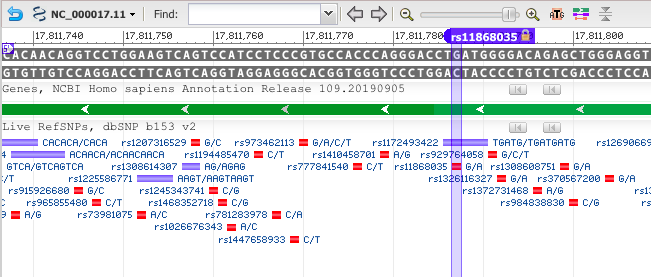
\includegraphics[scale=.5]{graphics/snps.png}
	\end{center}
	\caption{NCBI's Genomic regions, transcripts, and products.}
	\label{fig:ncbi}
\end{figure}

% good NCBI information video: https://www.youtube.com/watch?v=-dOQMiEtL8I

\subsubsection*{GitHub starter link}
\begin{center}
\color{red} \url{https://classroom.github.com/a/k4uhy6MT} \color{black}
\end{center}



To use this link, please follow the steps below.
\begin{itemize}
	\item Click on the link and accept the assignment.
	\item Once the importing task has completed, click on the created assignment link which will take you to your newly created GitHub repository for this lab.
	\item Clone this repository (bearing your name) and work on the practical locally.
	\item As you are working on your practical, you are to commit and push regularly. You can use the following commands to add a single file, you must be in the directory where the file is located (or add the path to the file in the command):
		\begin{itemize}
		\item {\tt git add -A}
		\item {\tt git commit -m ``Your notes about commit here''}
		\item {\tt git push}
	\end{itemize}

	Alternatively, you can use the following commands to add multiple files from your repository:
	\begin{itemize}
		\item {\tt git commit <}\emph{nameOfFile}\tt{> -m ``Your notes about commit here''}
		\item {\tt git push}
	\end{itemize}
\end{itemize}
%%%

Be sure to read the {\tt README.md} file in the GitHub Classroom repository for instructions on how to complete your first assignment.

% good reference on reading NCBI's gene data
% https://www.youtube.com/watch?v=-dOQMiEtL8I



\subsection*{Objectives}
\begin{itemize}
	\item To learn how to use a Web-based genomic databases and tools.
	\item To understand some of the types of information that are stored in PubMed databases.
	\item To learn how to use different interfaces to find and retrieve genomic information. 
%	\item To Learn how to write a program in python to load files using built-in control statements. 
\end{itemize}

%\vspace*{-.1in}
%\subsection*{Reading Assignment}
%\vspace*{-.1in}
%Chapter 1 in the \emph{Exploring Bioinformatics} textbook.

\vspace*{-.1in}
\subsection*{Locate your data on PubMed}
\vspace*{-.1in} 

\textbf{PubMed} (available at: \url{https://www.ncbi.nlm.nih.gov/pubmed/}), is a large, online, database resource containing information regarding DNA, genes, RNA, protein products, literature and graphical resources such as, \emph{Genomic regions, transcripts, and products}, as shown in Figure \ref{fig:ncbi}. These resources are curated for bioinformatics and biological science meaning that the information comes from an educated and factual basis. As written on their website, PubMed comprises more than 30 million citations for biomedical literature from MEDLINE, life science journals, and online books. Citations may include links to full-text content from PubMed Central and publisher web sites. This great resource provides much of the data that bioinformaticians may use during the course of their work in research.


\textbf{Single-nucleotide polymorphisms} ({SNPs, pronounced \emph{snips}) are DNA sequence variations occurring when a single nucleotide (i.e., adenine (A), thymine (T), cytosine (C), or guanine (G) in the genome, or other shared sequence) differs between members of a species or paired chromosomes in an individual. As mentioned in class, the appearance of these SNPs may be used to separate DNA samples from each other based on the presence or absence of a particular type of nucleotide.

For instance, the research group, Do \emph{et al.} \cite{do2011web} genotyped 3,426 PD patients and 29,624 healthy control individuals for 522,782 known simple nucleotide polymorphisms (SNPs). They identified 11 SNP sites where one allele was correlated with PD with a statistically significant frequency. Known (SNPs) in the human genome are recorded in the primary genomic database dbSNP, where each SNP has a unique accession number that identifies it. In this laboratory assignment you will investigate the genomic neighborhood of one of these SNPs with the accession number \emph{rs11868035}, which was identified by Do \emph{et al.} 


\vspace*{-.2in}

\subsection*{Part 1: PubMed's Online Resource}
\vspace*{-.1in}

Please locate the markdown file, {\tt writing/stepsAndQuestions.md} and follow the instructions to complete the thirteen (13) questions found in this file. 
\vspace*{-.2in}

\subsection*{Part 2: The Ethics of Online Information}
\vspace*{-.1in}

PubMed is a resource from which biological and health-sciences data may be located. A majority of the data on this site has been \emph{curated} by researchers, meaning that there is some form of credibility behind each piece of the site's information. For instance, the literature that PubMed offers has all been peer-reviewed to imply that a particular article's foundations, methods and conclusions were created using an educated, informed and logical conduct. Researchers who use the PubMed resource are therefore able to assume that the facts that they gain from the PubMed resource are real and worthy of their considerations for the determination of other types of truth from research.

There are sites online who freely offer media which has not been curated for faults and flaw. For this information there is no approval of any kind that the information may be used for any reason. Sadly, many consumers of this information apply this unconfirmed knowledge to their daily lives.


Please read the Washington Post article entitled, \emph{They turn to Facebook and YouTube to find a cure for cancer — and get sucked into a world of bogus medicine}, (\href{https://www.washingtonpost.com/lifestyle/style/they-turn-to-facebook-and-youtube-to-find-a-cure-for-cancer--and-get-sucked-into-a-world-of-bogus-medicine/2019/06/25/6df3ddae-7cdc-11e9-a5b3-34f3edf1351e_story.html}{article link}, \cite{Ohlheiser}), and complete the questions found in the file {\tt ethics/reflections.md}.



\color{red}
\vspace*{-.2in}
\subsection*{Required Deliverables}
\vspace*{-.1in}
    \begin{itemize}
     \item Your report from your adventures with NCBI's online resource: {\tt \color{red} writing/stepsAndQuestions.md \color{black}}
     \item Your reflection document to respond to the questions in the article: {\tt \color{red} ethics/reflections.md \color{black}}
    \end{itemize}
\color{black}


\noindent Please see the instructor if you have questions about assignment or its submission.

\bibliographystyle{plain}
\bibliography{allRefs}

%Article reference: Ohlheiser, Abby. \emph{They turn to Facebook and YouTube to find a cure for cancer — and get sucked into a world of bogus medicine}, The Washington Post, 25 June 2019

\end{document}

%%%% JUNK BIN %%%%
%%%% JUNK BIN %%%%
%%%% JUNK BIN %%%%
%%%% JUNK BIN %%%%
%%%% JUNK BIN %%%%
%%%% JUNK BIN %%%%






}% end of omitit{}

%%%%%%%%%%%%%%%
